\documentclass[tikz, border=1mm]{standalone}
\usepackage{tikz} 
\usetikzlibrary{arrows.meta}
\usepackage{pgfplots}

\pgfplotsset{compat=1.18}

\begin{document}

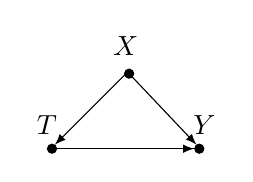
\begin{tikzpicture}

    % nodes (variables)
    %\node at (-3,0) {$e_{T}$};
    \node at (-2,0) {$T$};
    %\node at (-2,1) {$e_{X}$};
    \node at (-1,1) {$X$};
    \node at (0,0) {$Y$};
    %\node at (1,0) {$e_{Y}$};
    
	% edges
    %\draw[{Circle[open]}-{latex}](-3,-0.3) to (-2,-0.3); % e_{T} -> T
    %\draw[{Circle[open]}-{latex}](-2,0.65) to (-1,0.65); % e_{X} -> X
    \draw[{Circle}-{latex}{Circle}](-2,-0.3) to (0,-0.3); % T -> Y
    \draw[-{latex}](-0.95,0.7) to (-1.9,-0.25); % X -> T
    \draw[{Circle}-{latex}](-1,0.7) to (-0.1,-0.25); % X -> Y
    %\draw[{Circle[open]}-{latex}](1,-0.3) to (0,-0.3); % e_{Y} -> Y    

\end{tikzpicture}

\end{document}
